%%=============================================================================
%% Resultaten
%%=============================================================================

\chapter{Resultaten}
\label{ch:resultaten}

Om de verschillende modellen te testen, worden meerdere scenario’s gehanteerd.
Ten eerste wordt gebruikgemaakt van een testset met tien vragen waarvan de informatie beschikbaar is in de documentatie. Van elk model wordt verwacht dat het op iedere vraag een concreet antwoord geeft. Deze antwoorden worden vervolgens geëvalueerd met behulp van het test framework Ragas, waarbij vier verschillende meetcriteria worden toegepast.
\\[1em]
Het tweede testscenario bestaat uit het stellen van niet-triviale vragen waarvoor de informatie niet beschikbaar is in de documentatie. Dit scenario is vooral bedoeld om te onderzoeken of bepaalde modellen tekenen van hallucinaties vertonen.
\\[1em]
Als laatste worden enkele triviale vragen gesteld. Hierbij wordt getest of het model in staat is een juiste inschatting te maken door direct te antwoorden, zonder onnodige zoekopdrachten in de vector database.

\section{Evaluatie 1: Documentatiegebaseerde vragen}

Voor elk model werd een afzonderlijke vragenlijst opgesteld, waarbij de verwachte antwoorden zijn opgenomen in bijlage \ref{vragenlijst}.
De antwoorden die door de modellen zijn gegenereerd, zijn weergegeven in bijlage \ref{antwoordenlijst}.
In beide bijlagen zijn, uit overwegingen van gegevensbescherming, alle contactgegevens geanonimiseerd.
\\[1em]
Voor deze evaluatie wordt gebruikgemaakt van een testframework \textit{Ragas}. Tijdens de testen wordt voor iedere vraag de volgende informatie verzameld: de gebruikersinput, de opgehaalde context, het antwoord van de LLM en het verwachte antwoord. Op basis van deze gegevens gebruikt Ragas zelf een LLM om de dataset te beoordelen volgens de gekozen evaluatie criteria. In dit geval werd hiervoor het testmodel \texttt{gemma3:4b} gebruikt, omdat dit model een goede balans biedt tussen rekensnelheid, geheugengebruik en beoordelingskwaliteit. Hierdoor kon de evaluatie efficiënt worden uitgevoerd. Dit resulteert in een rapport waarin iedere vraag wordt beoordeeld op de verschillende criteria.
\\[1em]
De scores per vraag variëren tussen 0 en 1, waarbij een score van 1 een volledig correct antwoord representeert.
Binnen de categorie \textit{Faithfulness} geeft een score van 0{,}000 aan dat het model ten onrechte heeft nagelaten de retriever-tool te gebruiken, waardoor de opgehaalde context leeg bleef.
Voor de categorie \textit{Context Recall} kan dit in sommige gevallen juist het tegenovergestelde effect hebben: wanneer de opgehaalde context leeg is, kan het antwoord van het model toch een score van 1 behalen, mits het volledig aansluit bij de afwezigheid van context.
\\[1em]
De meetcriteria \textit{Faithfulness} beoordeelt hoe consistent het antwoord is met de opgehaalde context. \textit{Response relevancy} kijkt naar hoe relevant het antwoord is ten opzichte van de vraag. Onvolledige of overbodige informatie leidt hierbij tot een lagere score. \textit{Answer correctness} beoordeelt hoe correct het antwoord is in vergelijking met het verwachte antwoord, waarbij zowel feitelijke als semantische overeenkomsten worden meegenomen. \textit{Context recall} controleert in welke mate de benodigde informatie voor het antwoord aanwezig is in de opgehaalde context. Hoe groter de overlap tussen het juiste antwoord en de context, hoe hoger de score. Deze meetcriteria kijkt dus vooral naar hoe goed het model het ophaalproces aanstuurt.
\\[1em]
Op basis van deze evaluatie zijn de volgende resultaten vastgesteld:
\subsection{Llama3.1}

\begin{table}[H]
    \begin{tabular}{|l|c|c|c|c|}
        \hline
        \textbf{Vraag} & \textbf{Faithfulness} & \textbf{Response relevancy} & \textbf{Answer correctness} & \textbf{Context recall} \\
        \hline
        Vraag 1 & 1.000 & 0.000 & 0.225 & 0.500 \\
        Vraag 2 & 0.333 & 0.000 & 0.221 & 0.000 \\
        Vraag 3 & 0.385 & 0.000 & 0.223 & 0.500 \\
        Vraag 4 & 0.000 & 0.000 & 0.174 & 1.000 \\
        Vraag 5 & 1.000 & 0.863 & 0.212 & 0.125 \\
        Vraag 6 & 0.667 & 0.920 & 0.477 & 1.000 \\
        Vraag 7 & 0.500 & 0.000 & 0.205 & 1.000 \\
        Vraag 8 & 0.714 & 0.000 & 0.408 & 1.000 \\
        Vraag 9 & 0.500 & 0.932 & 0.391 & 1.000 \\
        Vraag 10 & 0.333 & 0.000 & 0.205 & 1.000 \\
        \hline
    \end{tabular}
    \caption{Resultaten per vraag op de vier meetcriteria van het Llama3.1 model.}
    \label{tab:resultaten_vragen_llama3.1}
\end{table}

\subsection{Llama3.2}

\begin{table}[H]
    \centering
    \begin{tabular}{|l|c|c|c|c|}
        \hline
        \textbf{Vraag} & \textbf{Faithfulness} & \textbf{Response relevancy} & \textbf{Answer correctness} & \textbf{Context recall} \\
        \hline
        Vraag 1  & 0.500 & 0.894 & 0.485 & 0.500 \\
        Vraag 2  & 0.333 & 0.000 & 0.220 & 0.000 \\
        Vraag 3  & 0.800 & 0.000 & 0.219 & 0.500 \\
        Vraag 4  & 0.571 & 0.863 & 0.196 & 0.833 \\
        Vraag 5  & 0.625 & 0.000 & 0.205 & 0.125 \\
        Vraag 6  & 0.857 & 0.000 & 0.194 & 1.000 \\
        Vraag 7  & 0.917 & 0.860 & 0.991 & 1.000 \\
        Vraag 8  & 0.833 & 0.953 & 0.212 & 1.000 \\
        Vraag 9  & 0.429 & 0.883 & 0.631 & 0.375 \\
        Vraag 10 & 0.333 & 0.000 & 0.207 & 1.000 \\
        \hline
    \end{tabular}
    \caption{Resultaten per vraag op de vier meetcriteria van het Llama3.2 model.}
    \label{tab:resultaten_vragen_llama3.2}
\end{table}

\subsection{Qwen2.5}

\begin{table}[H]
    \begin{tabular}{|l|c|c|c|c|}
        \hline
        \textbf{Vraag} & \textbf{Faithfulness} & \textbf{Response relevancy} & \textbf{Answer correctness} & \textbf{Context recall} \\
        \hline
        Vraag 1  & 0.750 & 0.000 & 0.485 & 0.500 \\
        Vraag 2  & 0.500 & 0.000 & 0.226 & 0.000 \\
        Vraag 3  & 0.929 & 0.000 & 0.229 & 0.500 \\
        Vraag 4  & 0.000 & 0.000 & 0.174 & 1.000 \\
        Vraag 5  & 0.000 & 0.000 & 0.180 & 0.000 \\
        Vraag 6  & 1.000 & 0.871 & 0.469 & 1.000 \\
        Vraag 7  & 0.000 & 0.000 & 0.176 & 1.000 \\
        Vraag 8  & 0.000 & 0.000 & 0.179 & 0.000 \\
        Vraag 9  & 0.000 & 0.000 & 0.176 & 0.556 \\
        Vraag 10 & 0.667 & 0.000 & 0.216 & 0.000 \\
        \hline
    \end{tabular}
    \caption{Resultaten per vraag op de vier meetcriteria van het Qwen2.5 model.}
    \label{tab:resultaten_vragen_qwen2.5}
\end{table}


\subsection{Qwen3}

\begin{table}[H]
    \begin{tabular}{|l|c|c|c|c|}
        \hline
        \textbf{Vraag} & \textbf{Faithfulness} & \textbf{Response relevancy} & \textbf{Answer correctness} & \textbf{Context recall} \\
        \hline
        Vraag 1  & 1.000 & 0.000 & 0.216 & 0.500 \\
        Vraag 2  & 1.000 & 0.000 & 0.224 & 0.000 \\
        Vraag 3  & 1.000 & 0.000 & 0.220 & 0.250 \\
        Vraag 4  & 0.857 & 0.000 & 0.203 & 0.000 \\
        Vraag 5  & 0.636 & 0.867 & 0.211 & 0.125 \\
        Vraag 6  & 0.750 & 0.874 & 0.571 & 1.000 \\
        Vraag 7  & 1.000 & 0.906 & 0.989 & 1.000 \\
        Vraag 8  & 0.556 & 0.000 & 0.411 & 1.000 \\
        Vraag 9  & 1.000 & 0.000 & 0.340 & 0.625 \\
        Vraag 10 & 1.000 & 0.935 & 0.636 & 1.000 \\
        \hline
    \end{tabular}
    \caption{Resultaten per vraag op de vier meetcriteria van het Qwen3 model.}
    \label{tab:resultaten_vragen_qwen3}
\end{table}


\subsection{Samenvatting}

Om de prestaties van de modellen per individuele metric te vergelijken, worden in figuur~\ref{fig:vergelijking_metrics} vier staafdiagrammen weergegeven: Faithfulness, Response relevancy, Answer correctness en Context recall.

\begin{figure}[H]
    \centering
    \begin{subfigure}{0.48\textwidth}
        \centering
        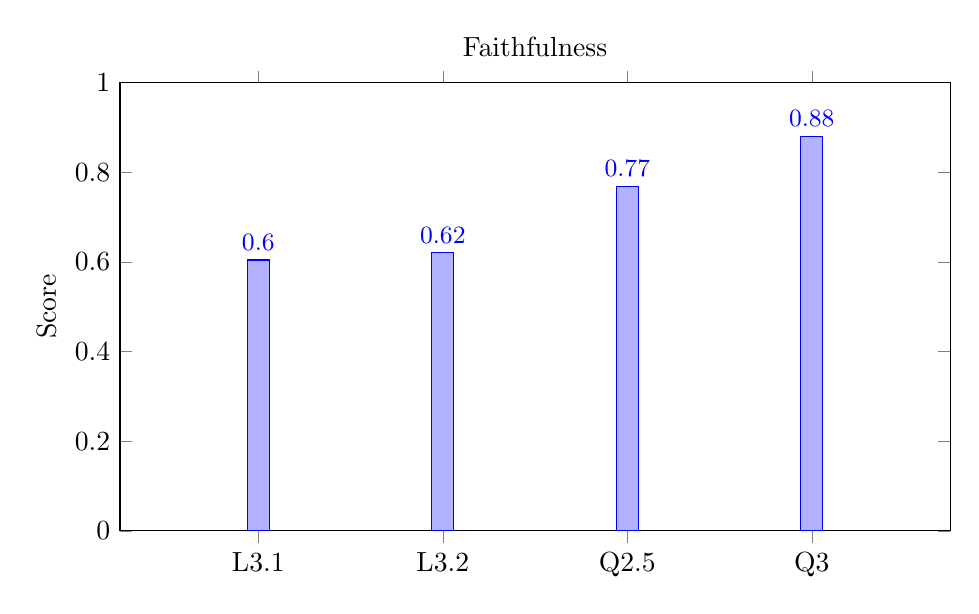
\begin{tikzpicture}
            \begin{axis}[
                ybar,
                ymin=0,
                ymax=1,
                bar width=8pt,
                width=\textwidth,
                height=0.6\textwidth,
                enlarge x limits=0.25,
                ylabel={Score},
                symbolic x coords={L3.1,L3.2,Q2.5,Q3},
                xtick=data,
                nodes near coords,
                nodes near coords align={vertical},
                every node near coord/.append style={font=\small},
                title={Faithfulness}
                ]
                \addplot coordinates {(L3.1,0.604) (L3.2,0.620) (Q2.5, 0.769) (Q3,0.880)};
            \end{axis}
        \end{tikzpicture}
    \end{subfigure}
    \hfill
    \begin{subfigure}{0.48\textwidth}
        \centering
        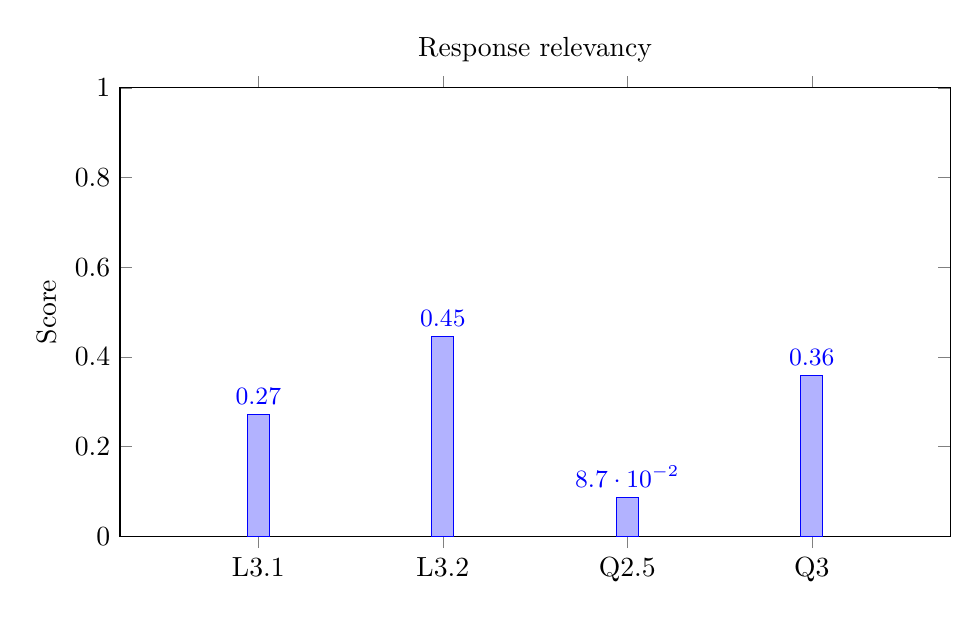
\begin{tikzpicture}
            \begin{axis}[
                ybar,
                ymin=0,
                ymax=1,
                bar width=8pt,
                width=\textwidth,
                height=0.6\textwidth,
                enlarge x limits=0.25,
                ylabel={Score},
                symbolic x coords={L3.1,L3.2,Q2.5,Q3},
                xtick=data,
                nodes near coords,
                nodes near coords align={vertical},
                every node near coord/.append style={font=\small},
                title={Response relevancy}
                ]
                \addplot coordinates {(L3.1,0.272) (L3.2,0.445) (Q2.5,0.087) (Q3,0.358)};
            \end{axis}
        \end{tikzpicture}
    \end{subfigure}
    
    \vspace{1em}
    
    \begin{subfigure}{0.48\textwidth}
        \centering
        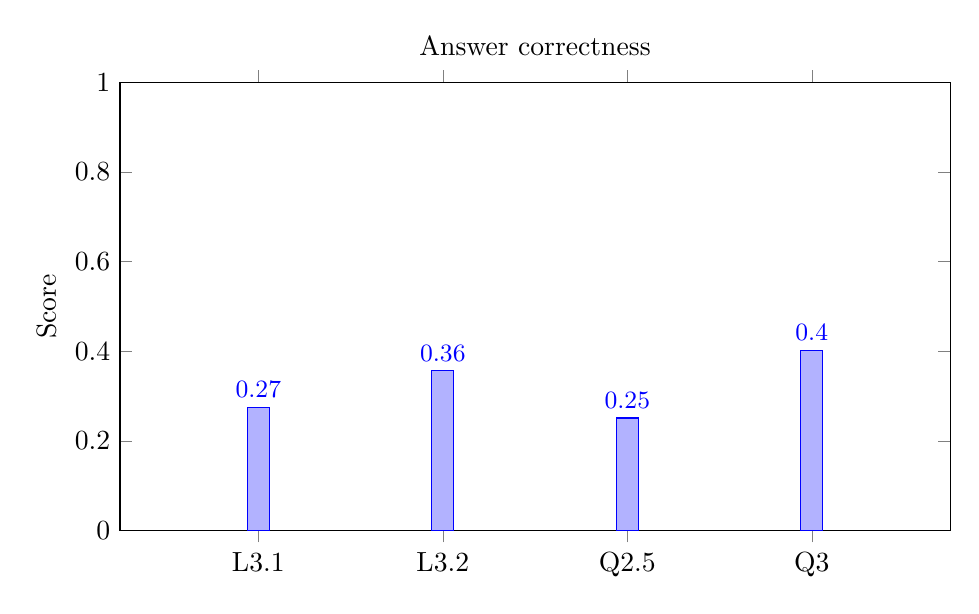
\begin{tikzpicture}
            \begin{axis}[
                ybar,
                ymin=0,
                ymax=1,
                bar width=8pt,
                width=\textwidth,
                height=0.6\textwidth,
                enlarge x limits=0.25,
                ylabel={Score},
                symbolic x coords={L3.1,L3.2,Q2.5,Q3},
                xtick=data,
                nodes near coords,
                nodes near coords align={vertical},
                every node near coord/.append style={font=\small},
                title={Answer correctness}
                ]
                \addplot coordinates {(L3.1,0.274) (L3.2,0.356) (Q2.5,0.251) (Q3,0.402)};
            \end{axis}
        \end{tikzpicture}
    \end{subfigure}
    \hfill
    \begin{subfigure}{0.48\textwidth}
        \centering
        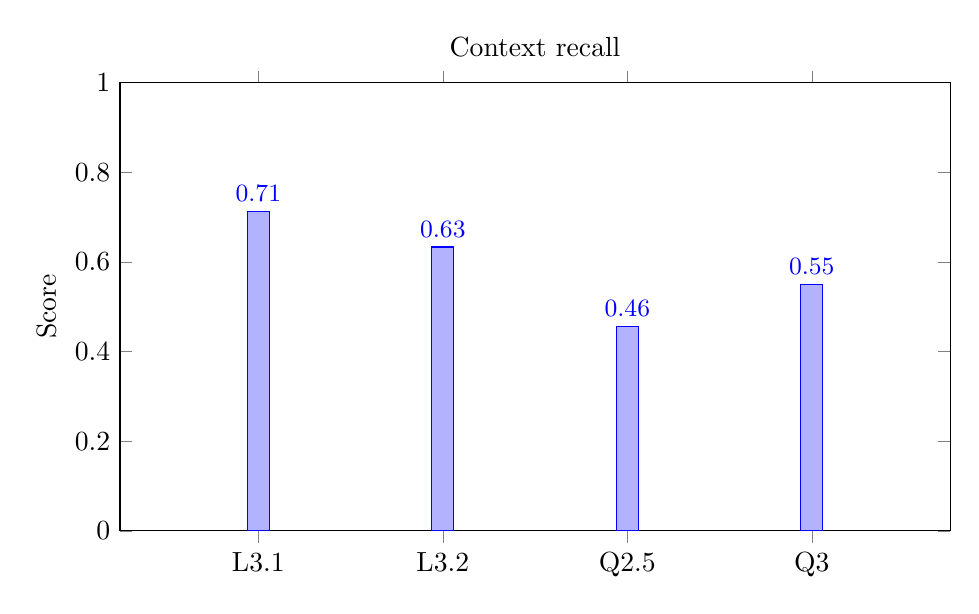
\begin{tikzpicture}
            \begin{axis}[
                ybar,
                ymin=0,
                ymax=1,
                bar width=8pt,
                width=\textwidth,
                height=0.6\textwidth,
                enlarge x limits=0.25,
                ylabel={Score},
                symbolic x coords={L3.1,L3.2,Q2.5,Q3},
                xtick=data,
                nodes near coords,
                nodes near coords align={vertical},
                every node near coord/.append style={font=\small},
                title={Context recall}
                ]
                \addplot coordinates {(L3.1,0.713) (L3.2,0.633) (Q2.5,0.456) (Q3, 0.550)};
            \end{axis}
        \end{tikzpicture}
    \end{subfigure}
    
    \caption{Vergelijking van de prestaties per metric voor alle modellen.}
    \label{fig:vergelijking_metrics}
\end{figure}

Gemiddeld over de vier categorieën scoren de modellen als volgt:

\begin{figure}[H]
    \centering
    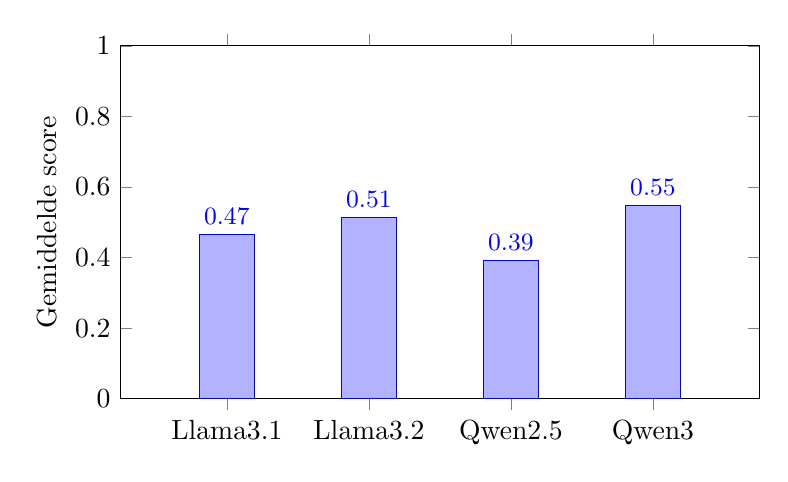
\begin{tikzpicture}
        \begin{axis}[
            ybar,
            ymin=0,
            ymax=1,
            bar width=20pt,
            width=0.8\textwidth,
            height=0.5\textwidth,
            enlarge x limits=0.25,
            ylabel={Gemiddelde score},
            symbolic x coords={Llama3.1,Llama3.2,Qwen2.5,Qwen3},
            xtick=data,
            nodes near coords,
            nodes near coords align={vertical},
            every node near coord/.append style={font=\small},
            ]
L            \addplot coordinates {(Llama3.1,0.466) (Llama3.2,0.514) (Qwen2.5,0.391) (Qwen3,0.548)};
        \end{axis}
    \end{tikzpicture}
    \caption{Gemiddelde score per model.}
    \label{fig:gemiddelde_score_per_model}
\end{figure}

\begin{table}[H]
    \begin{tabular}{|l|c|c|c|c|c|}
        \hline
        \textbf{Model} & \textbf{Faithfulness} & \textbf{Response relevancy} & \textbf{Answer correctness} & \textbf{Context recall} \\
        \hline
        \textbf{llama3.1} & 0.604 & 0.272 & 0.274 & \textbf{0.713} \\
        \textbf{llama3.2} & 0.620 & \textbf{0.445} & 0.356 & 0.633 \\
        \textbf{qwen2.5}  & 0.769 & 0.087 & 0.251 & 0.456 \\
        \textbf{qwen3}    & \textbf{0.880} & 0.358 & \textbf{0.402} & 0.550 \\
        \hline
    \end{tabular}
    \caption{Vergelijking van modelprestaties.}
    \label{tab:modelvergelijking}
\end{table}

Uit tabel \ref{tab:modelvergelijking} blijkt dat het model Qwen3 de hoogste scores behaalde voor faithfulness (0.880) en answer correctness (0.402), terwijl Llama3.2 het beste presteerde op response relevancy (0.445) en Llama3.1 op context recall (0.713).

\section{Evaluatie 2: Hallucinaties}


Bij deze test krijgt ieder model een set van 5 vragen voorgeschoteld. Geen van deze vragen komt voor in de documentatie (zie bijlage \ref{hallucinatie-resultaten} Dit heeft als doel om na te gaan welke modellen tekenen vertonen van hallucinaties en welke niet. 
\\[1em]
De vragenlijst is als volgt:

\begin{enumerate}
    \item Voor welke dienst is Jan Cabooter verantwoordelijk?
    \item Wat is de maximale bestandsgrootte (in MB) die via de repush voor RV kan worden verstuurd?
    \item Wat is de kost voor een Nationality change?
    \item Wat is de technical resource voor DQSS?
    \item Wat is het maximum aantal documenten die kunnen geraadpleegd worden bij myminfin
\end{enumerate}

\begin{table}[H]
    \begin{tabular}{|l|c|c|c|c|}
        \hline
        \textbf{Vraag} & \textbf{Llama3.1} & \textbf{Llama3.2} & \textbf{Qwen2.5} & \textbf{Qwen3} \\
        \hline
       Vraag 1 & Nee & Ja & Nee & Nee \\
       Vraag 2 & Nee & Ja & Ja & Ja \\
       Vraag 3 & Ja & Nee & Nee & Nee \\
       Vraag 4 & Nee & Ja & Nee & Nee \\
       Vraag 5 & Nee & Ja & Nee & Nee \\
        \hline
    \end{tabular}
    \caption{Resultaten hallucinatie test per model bij vragen die niet in de documentatie voorkomen (Ja = hallucinatie, Nee = geen hallucinatie)}
\end{table}

\noindent\textbf{Samenvatting:}  
\begin{table}[H]
    \begin{tabular}{|l|c|}
        \hline
        \textbf{Model} & \textbf{Hallucinatie (\%)} \\
        \hline
        Llama3.1 & 1/5 (20\%) \\
        Llama3.2 & 4/5 (80\%) \\
        Qwen2.5  & 1/5 (20\%) \\
        Qwen3    & 1/5 (20\%) \\
        \hline
    \end{tabular}
    \caption{Samenvatting hallucinatie test}
\end{table}

Uit de resultaten blijkt dat Llama3.2 in 80\% van de gevallen hallucinaties vertoonde, terwijl de overige modellen dit slechts in 20\% van de gevallen deden.


\section{Evaluatie 3: Triviale vraagstelling}

Tijdens deze test kreeg ieder model een reeks van vijf triviale vragen voorgelegd. De resultaten werden bepaald door de stacktrace van ieder model te analyseren. Op die manier werd vastgesteld of het model de vraag direct beantwoordde of eerst onnodig RAG uitvoerde (zie bijlage \ref{triviale-vragen-resultaten}).
\\[1em]
De vragenlijst is als volgt:

\begin{enumerate}
    \item Hallo hoe gaat het?
    \item Hoeveel dagen zitten er in een week?
    \item Wat is 2 + 2?
    \item In welk land ligt Parijs?
    \item Hoeveel minuten zitten er in een uur?
\end{enumerate}

\begin{table}[H]
    \centering
    \begin{tabular}{|l|c|c|c|c|}
        \hline
        \textbf{Vraag} & \textbf{llama3.1} & \textbf{llama3.2} & \textbf{Qwen2.5} & \textbf{Qwen3} \\
        \hline
        Hallo hoe gaat het? & Nee & Nee & Ja & Ja \\
        Hoeveel dagen zitten er in een week? & Nee & Nee & Ja & Ja \\
        Wat is 2 + 2? & Nee & Nee & Ja & Ja \\
        In welk land ligt Parijs? & Nee & Nee & Ja & Ja \\
        Hoeveel minuten zitten er in een uur? & Nee & Nee & Ja & Ja \\
        \hline
    \end{tabular}
    \caption{Resultaten correct gebruik van de graaf per model bij triviale vragen (verwacht gedrag: direct antwoord, geen RAG)}
\end{table}

\noindent\textbf{Samenvatting:}  
\begin{table}[H]
    \begin{tabular}{|l|c|}
        \hline
        \textbf{Model} & \textbf{Correct (\%)} \\
        \hline
        Llama3.1 & 0/5 (0\%) \\
        Llama3.2 & 0/5 (0\%) \\
        Qwen2.5  & 5/5 (100\%) \\
        Qwen3    & 5/5 (100\%) \\
        \hline
    \end{tabular}
    \caption{Samenvatting van correct gebruik van de graaf per model}
\end{table}

Uit de resultaten blijkt dat Qwen2.5 en Qwen3 alle triviale vragen direct beantwoordden, terwijl Llama3.1 en Llama3.2 in alle gevallen onnodige RAG uitvoerden.

